
\chapter{Analysis And Results}
\label{ch:Results}
%Deep thoughts go here.
This search is to attempt to observe the FCNC decay of a top quark $t \rightarrow q \gamma$ or to set an upper limit on the branching ratio of this decay process if no observation occurs.  As there is no significant excess of events in the collected data an upper limit on the branching ratio is set.  This chapter will discuss  the methods used to set the upper limit on the branching ratio as well as the systematic uncertainties within the experiment.   This chapter contains material coauthored by the ATLAS Collaboration.  I took advantage of the common tools developed by the ATLAS Collaboration for fitting and limit setting for the final results presented in this chapter.

\section{Systematic Uncertainties}
\label{sec:NPUncertainties}
Various sources of uncertainty are considered for any analysis in high energy physics.  Statistical and systematic uncertainties are studied and propagated through to the final upper limit set on the branching ratio.  The statistical errors are related to the amount of data collected or MC events that are available and created for analysis.  More data events or more MC simulated events lead to a smaller statistical error due to random fluctuations of stochastic processes.  In this section the systematic errors will be discussed.  Systematic errors are derived from limitations from detector construction or a lack of complete understanding of physics objects or algorithms used in reconstruction.  Some sources of systematic uncertainties are provided centrally within ATLAS from studies carried out by other analysis teams such as errors on the jet energy resolution (JER) or luminosity amongst others. Other sources are particular to the analysis such as errors propagating from deriving data-driven backgrounds as discussed in the previous chapter.
This section will briefly introduce and discuss the theoretical systematic uncertainties considered in this analysis including the modeling and experimental uncertainties as well as a discussion on systematic smoothing, symmetrization, and pruning used in the final fit. 

\subsection{Theoretical uncertainties}
\begin{description}
\item[\textbf{Cross Section}:]  Various cross sections for MC samples are separately varied up and down by one standard deviation for each process: $t\bar{t}$ ($\pm5.6\%$ \cite{ttXSec}), $t\bar{t}+\gamma$ ($\pm 8.0\%$ \cite{ATLAS:2018pmj}), single top(t-channel top $^{+4.0\%}_{-3.4\%}$, t-channel anti-top $^{+5.0\%}_{-4.5\%}$, s-channel top $^{+3.6\%}_{-3.1\%}$, s-channel anti-top $^{+4.8\%}_{-4.3\%}$, tW-channel $\pm 5.3\%$ \cite{SingleTopXSec}), V+jets ($\pm5\%$ \cite{VXSec}), and diboson VV ($\pm 6\%$ \cite{VXSec}).  
%Uncertainties on the prompt photon contribution from W/$t\bar{t}$+jets+$\gamma$ enter the fit as other nuisance parameters as the normalization is allowed to vary in the fit.

\item[\textbf{Renormalization and Factorization Scale}:]  The effect of the choice of renormalization and factorization scales ($\mu_r$ and $\mu_f$) is estimated varying them independently or simultaneously up and down by a factor of 2 compared to the nominal value.  This is done using event weights and the maximum and deviations from the nominal are taken to be the up and down variations.

\item[\textbf{PDF Uncertainty}:]  The PDF uncertainty is estimated using the PDF4LHC15 error set which contains 30 eigen variations which enter the fit as individual nuisance parameters.

\item[\textbf{Initial and Final State Radiation}:] The effects of ISR are estimated by decreasing the total QCD radiation activity in the events.  These variations are available for single top and $t\bar{t}$ processes.  For single top processes the A14 tune is varied up (down) using the event weight Var3cUp (Var3cDown) and dividing (multiplying) $\mu_r$ and $\mu_f$ by a factor of 2.  For $t\bar{t}$ processes a sample with parameter $h_\text{damp}=3m_\text{top}$ is used in the same manner varying Var3cUp while the down variation uses event weights in the nominal sample.   FSR uncertainties are estimated varying parameters using the A14 tune by varying event weight (Var2) up and down. %Change if not using single top information

%\item[\textbf{Normalization of Prompt Photon Contribution}:]  The normalization of the prompt photon contributions that stem from the W+jets+$\gamma$ and $t\bar{t}$+jets+$\gamma$, the major backgrounds, enter the fit as free floating nuisance parameters.

\item[\textbf{$\textbf{t}\bar{\textbf{t}}$ Matrix Element and Shower Generator}:]  To estimate the uncertainty based on the choice of MC generator and showering algorithm used to create the nominal sample (\textsc{Powheg-Box + Pythia}) is replaced by using samples generated using \textsc{MadGraph5\_}a\textsc{MC@NLO + Pythia} and \textsc{Powheg-Box + Herwig}.
\end{description}

\subsection{Experimental Uncertainties}
\begin{description}
\item[\textbf{Luminosity}:] The uncertainty in the combined 2015--2018 integrated luminosity is 1.7  \cite{ATLAS-CONF-2019-021}, obtained using the LUCID-2 detector \cite{LUCID2} for the primary luminosity measurements using x-y beam separation scans.

\item[\textbf{Pile-up}:]  Events are re-weighted in the MC samples to match the number of interactions per bunch crossing in data.  Systematic uncertainties for pile-up are evaluated by scaling these distributions up and down.

\item[\textbf{Lepton Identification and Trigger}:]   Lepton efficiencies contain the trigger, reconstruction, identification, and isolation efficiencies.  Scale factors are used to correct any deviation from data in the MC simulation.  Correction factors are derived from $Z\rightarrow ll$ and $J/ \psi \rightarrow ll$ decays for electrons \cite{ElectronID} and muons \cite{MuonID}.

\item[\textbf{Lepton Energy Scale and Resolution}:]  The lepton energy (momentum) is calibrated using MC -based techniques.  Correction factors derived from dileptonic Z boson decay channels are applied to account for detector calibration mismodeling.  For electrons, the energy scale and resolution are calculated together with photons as the EGamma energy scale and resolution.  Various efficiencies are derived for the EGamma scale and resolution, e.g., varying the amount of material in front of the calorimeters, using various MC generators, and considering varying background fits \cite{ElectronID, PhotonID}.
\item[\textbf{Photon Efficiency}:]  Scale factors for isolation are measured as described in Ref. \cite{Lesage:2017uzg} while additional scale factors for the photon ID efficiency are derived for photons using enriched $Z\rightarrow ee$ events where the similarity between electrons and photons in our detector is exploited using the matrix method as described in Section \ref{sec:FakePho}. These sets of scale factors are combined into a single set that is applied to MC simulation based on photon information.

\item[\textbf{Photon Energy Scale and Resolution}:]  Photon energy scale and resolution are calculated together with electron energy scale and resolution.

\item[\textbf{Jet Energy Scale}:] The jet energy scale (JES) and its uncertainty are derived using combinations of measurements in both simulation and data.  The \textit{CategoryReduction} reduction parameter set (30 nuisance parameters) are varied up and down and used for categories such as \textit{in-situ} jet energy corrections, flavor composition and response, $\eta$ inter-calibration, b-jet energy scale, and pile-up.

\item[\textbf{Jet Energy Resolution}:] The jet energy resolution (JER) is measured independently for data and MC using two techniques \cite{ATL-PHYS-PUB-2015-015} which results in 8 separate nuisance parameters.  These nuisance parameters are one-sided, as such the uncertainty is symmetrized.

%\item[\textbf{Jet Flavor Fraction}:]  Uncertainty arising from jet flavor composition the ratio of light-quark initiated to gluon-initiated jets is varied.  Nominally a 50:50 ratio is assumed with an uncertainty of 100\%.

\item[\textbf{Jet Vertex Tagging}:]  The cut on the jet vertex tagging (JVT) discriminant is varied up and down \cite{JetJVT} and the certainty on the JVT scale factor is calculated and then propagated through this analysis.

\item[\textbf{b-tagging}:]  Efficiencies for the various b-tagging working points are measured in data, and scale factors are derived for simulation depending on the jet flavor.  The uncertainties on these scale factors are provided by the Flavor Tagging group for b, c, and light jets.

\item[\textbf{$\slashed{E}$ Uncertainties}:]  Uncertainties on the lepton, photon, jet scale and resolution are propagated through to the missing transverse energy.  As such the impact on the $\slashed{E}$ uncertainty is estimated when evaluating the shift on the other variables.

\item[\textbf{Further Background Estimation}:] Uncertainties on the data-driven scale factors calculated for this analyis as described in Section \ref{sec:Fakes} are applied and the scale factors are varied up and down by one standard deviation.

\end{description}

\subsection{Symmetrization, Smoothing, and Pruning of Systematic Uncertainties}

Symmetrization and smoothing are methods used to minimize statistical fluctuations in various systematic sources.  Symmetrization centers the systematic uncertainty around a mean value and smoothing averages the expected number of events across bins in order to remove statistical fluctuations.

\subsubsection{Symmetrization}
Two-sided symmetrization is performed when up and down variations are provided for any given systematic.  The difference between these variations is calculated and the half sum of the absolute deviations from the nominal is taken as a symmetric variation:
\[ \text{ Symmetric Variation } = \frac{|\text{up} - \text{nominal}| +|\text{down}-\text{nominal}|}{2}  \]
The nominal value is then varied up and down by this symmetrized value.  However, if only an up or a down variation is provided for a systematic one-sided symmetrization is used by mirroring the absolute deviation about the nominal value.  Experimental systematic sources are generally symmetrized while signal and background modeling contributions are not.

\subsubsection{Smoothing}
Smoothing is a technique used to average statistics across bins.  This prevents large statistical spikes in many systematic uncertainties that are expected to provide small contributions.  The smoothing algorithm depends on two parameters: the tolerance and the maximal number of slope changes taking advantage of bin and neighboring bin information.  Distributions are rebinned until the statistical uncertainty of each bin is below the tolerance and then the number of slope changes in the distribution is checked.  If the number of slope changes is smaller than the threshold of four, then the distribution is kept, or else the first step is performed again with the tolerance value halved.  The smoothing algorithm 353QH \cite{Friedman:695770} is run to avoid artificially flat uncertainties being introduced in the first two steps.  All uncertainties are smoothed unless stated otherwise.  Smoothing does not change the overall normalizations of the uncertainty.

\subsubsection{Pruning}
\label{sec:Pruning}
\textit{Pruning} uncertainties is done in order to reduce the number of nuisance parameters (NP) and stabalize the fit.  Uncertainties that would only have a small impact on the end result are removed.  An initial fit is calculated for each NP using the $\pm 1 \sigma$ variation, and if the effect on the uncertainty is less than the given threshold of 1\%, the contribution is removed from further fits. %Change to match final value on % threshold

\section{Statistical Treatment of Results}
\label{sec:StatTreatment}
A profile likelihood fit is performed on the SR.  The \textbf{TRExFitter} framework \cite{TRExFitter} was used for this analysis which provides a framework built upon existing code such as the \textbf{RooStats} project\cite{Moneta:2010pm}.
Following \cite{Lista:2016chp} as well as the fit preformed in \cite{GregorFCNC} a likelihood function, $\mathcal{L}$, can be defined generally in the following manner:
\[ \mathcal{L} = \mathcal{L}(\mu,\theta|\overrightarrow{x})
\]
where the parameter $\mu$ is defined as the signal strength and $\theta$ as the set of nuisance parameters for the systematic uncertainties.  The parameter of interest in the fit is proxied as  $\overrightarrow{x}$.  The likelihood is computed using the following:
\[ \mathcal{L} = \displaystyle\prod_{r}^{N_\text{regions}}  \displaystyle\prod_{i}^{N_\text{r,bins}} P(N_{r,i}|N_{r,i}^\text{s} + \displaystyle\sum_{b}^{N_\text{bkg}}N_{r,i}^\text{b}) \displaystyle\prod_{j}^{N_\text{NP}} G(x|1,\sigma_{j})
\]
using the following parameters:
\begin{itemize}
\item $N_{\text{regions}}$ is the number of regions considered in the fit
\item $N_\text{r,bins}$ is the number of bins in region $r$
\item $r$ is the index that runs over each of the different regions
\item $i$ is the index that runs over the number of bins in the region being considered
\item $P(x|\lambda)$ is the Poisson function with a mean $\lambda$
\item $N_\text{r,i}$ is the observed number of events in bin $i$ of region $r$
\item $N_\text{r,i}^\text{s}$ is the expected number of signal events in bin $i$ of region $r$
\item $N_\text{bkg}$ is the number of background processes that are considered in the fit
\item $b$ is the index that runs over all cataeories of backgrounds considered
\item $N_\text{r,i}^\text{b}$ is the expected number of events of background $b$ in bin $i$ of region $r$
\item $N_\text{NP}$ is the total number of nuisance parameters (NPs) considered in the fit
\item $j$ is the index that runs over the number of NPs
\item $G(x|\mu,\sigma_{j})$ is a Gaussian function with mean $\mu$ and width $\sigma_\text{j}$ for the source of systematic uncertainty $j$ (this Gaussian is replaced with a Poisson function for statistical uncertainties due to MC statistics)
\end{itemize}

The signal strength, $\mu$, enters the likelihood as
\[ N_\text{r,i}^\text{s} = \mu \cdot N_\text{input,r}^\text{s} \cdot \rho_\text{r,i}
\]
with the number of signal events in region $r$, $N_\text{input,r}^\text{s}$ scaled using the effective cross section $\sigma_\text{eff}^\text{coup}$ and $\rho_\text{r,i}$, the fraction of signal events in the respective bin $i$ and region $r$. 

The decay mode effective cross section is given by:
\[\sigma_\text{eff, input}^\text{decay} = 2\times \sigma(pp\rightarrow t\bar{t}) \times \mathcal{B}(t\rightarrow Wb) \times \mathcal{B}(W\rightarrow l \nu)\times \mathcal{B}_\text{input}(t \rightarrow q \gamma)
\]
where $\sigma(pp\rightarrow t\bar{t}) =831.76$ pb, $\mathcal{B}(t\rightarrow bW) \approx1$, and $\mathcal{B}(W\rightarrow l \nu) =32.58\%$ .  The effective cross sections and couplings in the signal region are shown assuming the branching ratio to the FCNC decay mode $\mathcal{B}(t\rightarrow q \gamma) = 10^{-3}$ for q=u,c.  This implies that the total effective cross section used for the FCNC signal samples, $\sigma_\text{eff, input}^\text{decay}$, is 542 fb.  The final states of this analysis include both up type quark decay modes and the assumption is made that $\mathcal{B}(t\rightarrow u\gamma)$=$\mathcal{B}(t\rightarrow c\gamma)$.  As can be seen in figures of the Signal Region distributions in Section \ref{sec:SRPlots} the single top event rate is around 7\% of the total MC background.  Due to this the effect of the production mode ($u\rightarrow t\gamma$) is not further considered, as the final state for single top production with an association photon has significant kinematic differences to the regions in this analysis.  These events would appear as a further subset of the single top background.  Reconstructing an invariant mass around the top quark mass from the photon and the leading light jet is a key input to the neural network discriminator.  This is unlikely to occur in the production mode.

A profile likelihood approach for treatment of nuisance parameters\cite{Cowan:2010js} (systematic uncertainties presented in Section \ref{sec:NPUncertainties}) is used.

Physically this signal strength can be interpreted as the ratio of the signal cross section to the predicted signal cross section.  However if both the decay mode and production (prod) mode are considered then we can interpret $\mu$ as 
\[\mu = \frac{N_\text{fit}^\text{decay} + N_\text{fit}^\text{prod.}}{N_\text{input}^\text{decay} + N_\text{input}^\text{prod.}}
\]then it follows that 
\[\mu = \frac{\epsilon^\text{decay}\times \mathcal{A}^\text{decay} \times \sigma^\text{decay}_\text{eff, fit}\times L+\epsilon^\text{prod.}\times \mathcal{A}^\text{prod.} \times \sigma^\text{prod.}_\text{eff, fit} \times L}{\epsilon^\text{decay}\times \mathcal{A}^\text{decay} \times \sigma^\text{decay}_\text{eff, input} \times L+\epsilon^\text{prod.}\times \mathcal{A}^\text{prod.} \times \sigma^\text{prod.}_\text{eff, input}\times L}
\]
where the fitted (input) number of signal events per coupling (production/decay) $N_\text{fit (input)}^\text{coupling}$, the signal efficiencies $\sigma^\text{coupling}$, the detector acceptances $\mathcal{A}^\text{coupling}$, the fitted (input) effective cross sections $\sigma_\text{eff,fit(input)}^\text{coupling}$, and the luminosity $L$.  If it is then assumed that the detector acceptances and signal efficiencies are independent from the coupling strength and the fact that the signal samples have the same dependence on the coupling strength ($\sigma_\text{eff}^\text{decay}/ \sigma_\text{eff}^\text{prod.} = \text{constant}$), the expression for the signal strength can be simplified to the following form:
\[ \mu = \frac{\sigma_\text{eff,fit}^\text{decay}}{\sigma_\text{eff,input}^\text{decay}}=\frac{\sigma_\text{eff,fit}^\text{prod.}}{\sigma_\text{eff,input}^\text{prod.}}
\]

The background-only hypothesis is fulfilled when $\mu=0$.
For this search the signal strength can be classified in terms of the branching ratio (BR)

\[ \mu = \frac{\mathcal{B}(t\rightarrow q\gamma) \times \mathcal{B}(t\rightarrow Wb)}{\mathcal{B}_\text{input}(t\rightarrow q\gamma) \times \mathcal{B}_\text{input}(t\rightarrow Wb)}
\]
Under the assumption that the top quark nominally decays only to a b quark and a W boson ($\mathcal{B}(t\rightarrow bW)=1$) and the FCNC decay mode being searched is small ($\mathcal{B}(t\rightarrow q\gamma) << \mathcal{B}(t\rightarrow bW)$) this can be rewritten as 
\[ \mu = \frac{\mathcal{B}(t\rightarrow q\gamma) \times|1-\mathcal{B}(t\rightarrow q\gamma)|}{\mathcal{B}_\text{input}(t\rightarrow q\gamma) \times|1-\mathcal{B}_\text{input}(t\rightarrow q\gamma)|}
\]
\[ \mu \approx \frac{\mathcal{B}(t\rightarrow q\gamma)}{\mathcal{B}_\text{input}(t\rightarrow q\gamma)}
\]
Values of $\mu$ between 0 (background-only hypothosis) and 2 (2x the nominal branching ratio) are tested in order to calculated expected and observed limits using the $\text{CL}_\text{s}$ technique\cite{Read:2002hq} and presented in Section \ref{sec:Limits}.  The $\text{CL}_\text{s}$ technique makes use of a test statistic based on the negative log likelihood motivated by  Wilks' theorem that allows approximate aymptotic behavior $-2 \text{ln} \mathcal{L}(\mu)$ as a $\chi^2$ goodness of fit \cite{Wilks:1938dza}. %Change - maybe move?




\section{Nuisance Parameters}
The statistical analysis allows the uncertainties discussed in Section \ref{sec:NPUncertainties} to enter into the fits as nuisance parameters (NPs).  Each of these NPs is considered in all of the fit regions independently and dropped (pruned away) if its effect is less than 1\%.  Many of the parameters are dropped and for some only the normalization or the shape impact is dropped.  A large number of NPs are considered for each region and include theory, experimental, and modeling uncertainties.  Various plots showing which nuisance parameters are kept and dropped, pull values for the nuisance parameters, the bin by bin $\gamma$ normalization factors, the goodness of fit, and correlation matrix between nuisance parameters are presented in this section for the best fit regions.

%\subsection{$e$+jets Channel}
\begin{figure}[h!]
	\centering
	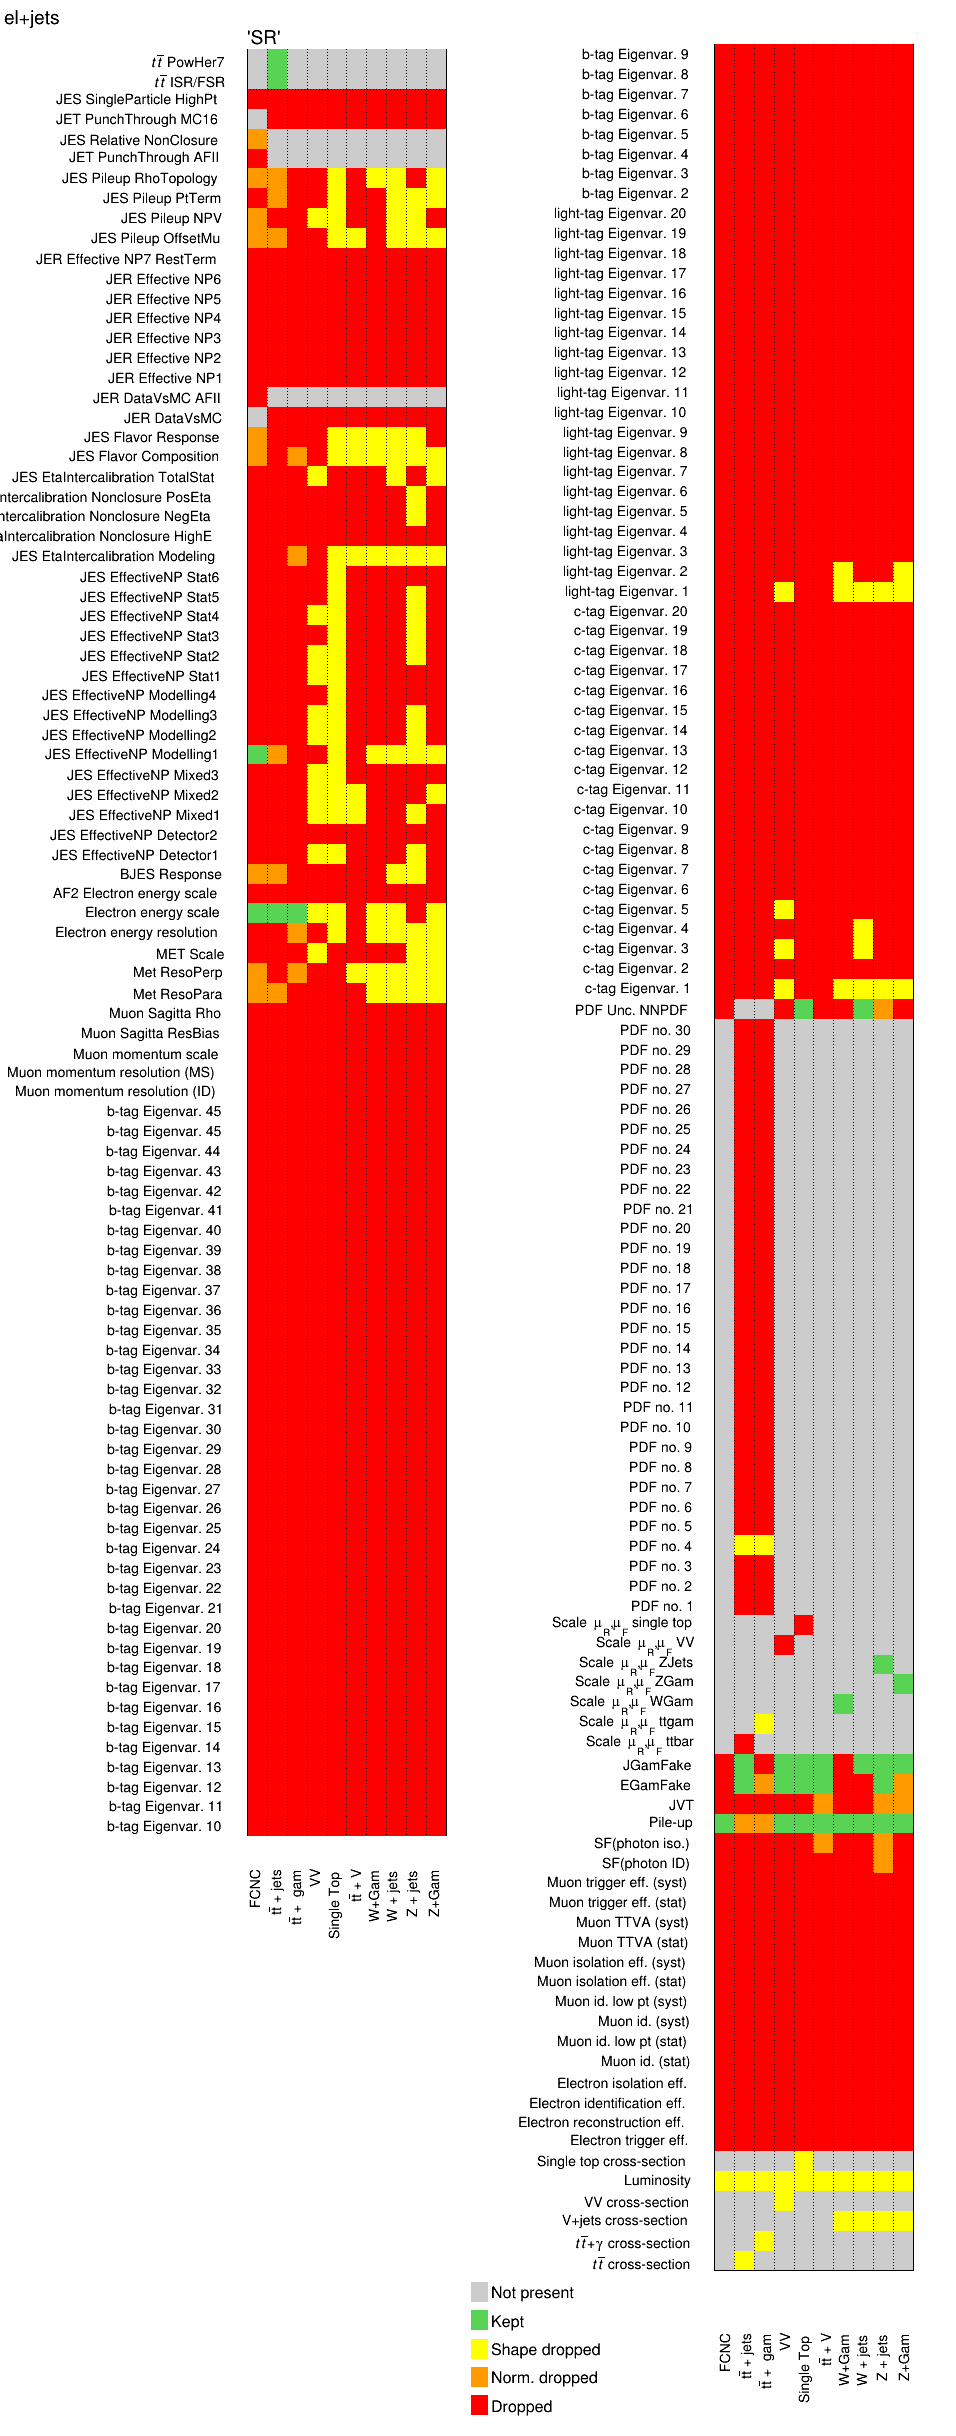
\includegraphics[width=.5\columnwidth]{../ThesisImages/RegionPlots/FinalRegions/Systematics/MQGamEJetPHptMJet/FCNC_All_ejets/Pruning.png}
	\caption[Nuisance parameters after pruning for $e$+jets channel]{Overview of nuisance parameters after pruning for the $e$+jets channel.  If shape or normalization impacts are smaller than 1\% that part of the nuisance parameter will be dropped in the final fit.}
	\label{fig:Pruningejets}
\end{figure}

\begin{figure}[h!]
	\centering
	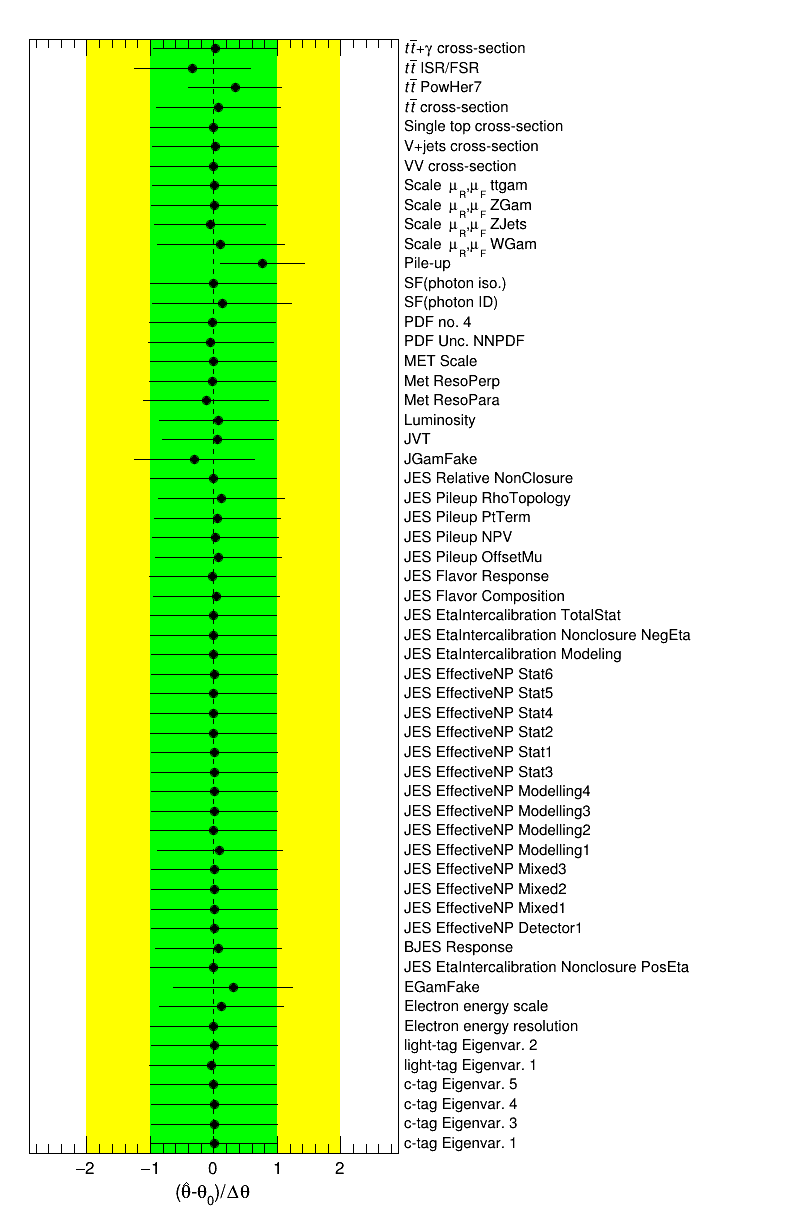
\includegraphics[width=.5\columnwidth]{../ThesisImages/RegionPlots/FinalRegions/Systematics/MQGamEJetPHptMJet/FCNC_All_ejets/NuisPar.png}
	\caption{Pull values for the various nuisance parameters considered in the fit for the $e$+jets channel.}
	\label{fig:NPejets}
\end{figure}

\begin{figure}[h!]
	\centering
	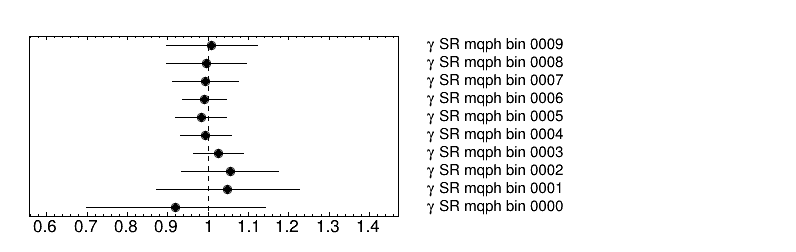
\includegraphics[width=.5\columnwidth]{../ThesisImages/RegionPlots/FinalRegions/Systematics/MQGamEJetPHptMJet/FCNC_All_ejets/Gammas.png}
	\caption{Bin by bin normalization $\gamma$ factors used in each region for the $e$+jets channel.}
	\label{fig:Gammasejets}
\end{figure}

\begin{figure}[h!]
	\centering
	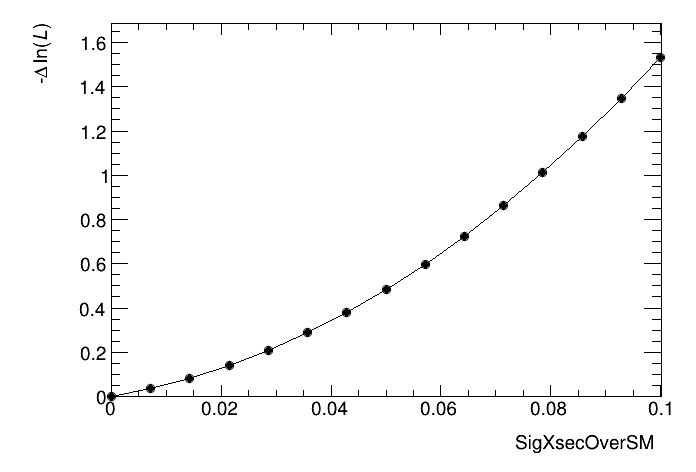
\includegraphics[width=.5\columnwidth]{../ThesisImages/RegionPlots/FinalRegions/Systematics/MQGamEJetPHptMJet/FCNC_All_ejets/LHoodPlots/NLLscan_SigXsecOverSM.png}
	\caption{Negative-log likelihood (goodness of fit) as a function of signal strength using data in all regions for the $e$+jets channel.}
	\label{fig:NLLejets}
\end{figure}

\begin{figure}[h!]
	\centering
	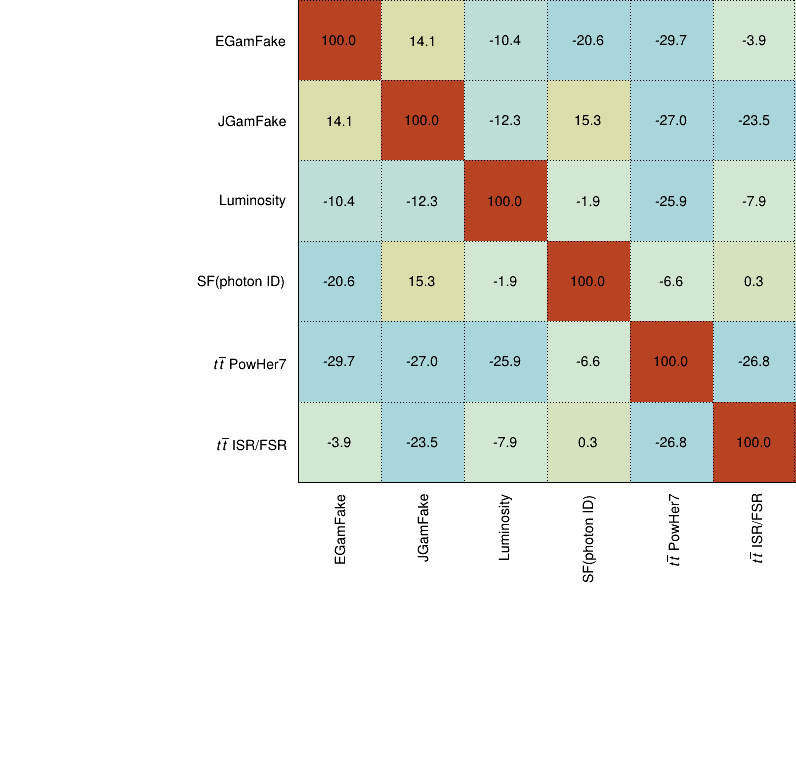
\includegraphics[width=.5\columnwidth]{../ThesisImages/RegionPlots/FinalRegions/Systematics/MQGamEJetPHptMJet/FCNC_All_ejets/CorrMatrix.png}
	\caption[Correlation matrix  with at least one coefficient above 20\% for $e$+jets channel]{Correlation matrix  with at least one coefficient above 20\% for $e$+jets channel. }
	\label{fig:Correjets}
\end{figure}

%% NB: add to main document: 
% \usepackage{siunitx} 
% \sisetup{separate-uncertainty,table-format=6.3(6)}  % hint: modify table-format to best fit your tables
\begin{table}[htbp]
\begin{center}
\footnotesize
\begin{tabular}{|l|S|S|S|}
\hline 
 & {'=1b,\geq 2j,=1\gamma'} & {'=0b,\geq 2j,=1\gamma'} & {'\geq 1 b,=1 \gamma , NN<Cut '}\\
\hline 
  FCNC   & 182.02 \pm 17.9455 & 118.773 \pm 11.7529 & 100.454 \pm 9.97274 \\ 
  t#bar{t} + jets   & 38.4403 \pm 4.96112 & 382.019 \pm 39.1136 & 1346.35 \pm 136.369 \\ 
  t#bar{t} +  gam   & 35.037 \pm 5.83114 & 236.41 \pm 38.4648 & 917.344 \pm 148.772 \\ 
  VV   & 0.71869 \pm 0.488437 & 80.4439 \pm 8.99439 & 5.75413 \pm 0.976033 \\ 
  Single Top   & 6.99979 \pm 1.62461 & 47.9589 \pm 6.09528 & 123.143 \pm 12.8614 \\ 
  t#bar{t} + V   & 0.272368 \pm 0.0624668 & 4.27229 \pm 0.39692 & 23.3092 \pm 1.67279 \\ 
  W+Gam   & 13.3192 \pm 2.65117 & 1984.1 \pm 169.111 & 140.108 \pm 15.0575 \\ 
  W + jets   & 4.67344 \pm 2.55462 & 899.99 \pm 128.251 & 53.174 \pm 10.3998 \\ 
  Z + jets   & 2.76455 \pm 0.993807 & 395.313 \pm 51.2636 & 33.591 \pm 4.12466 \\ 
  Z+Gam   & 1.62655 \pm 0.362593 & 271.217 \pm 21.0449 & 25.8642 \pm 3.48945 \\ 
\hline 
  Total background  & 103.852 \pm 6.43461 & 4301.72 \pm 126.013 & 2668.64 \pm 72.2158 \\ 
\hline 
\end{tabular} 
\caption{Yields of the analysis} 
\end{center} 
\end{table} 
%SR_mqph_syst_postFit}
%\subsection{$\mu$+jets Channel}
\begin{figure}[h!]
	\centering
	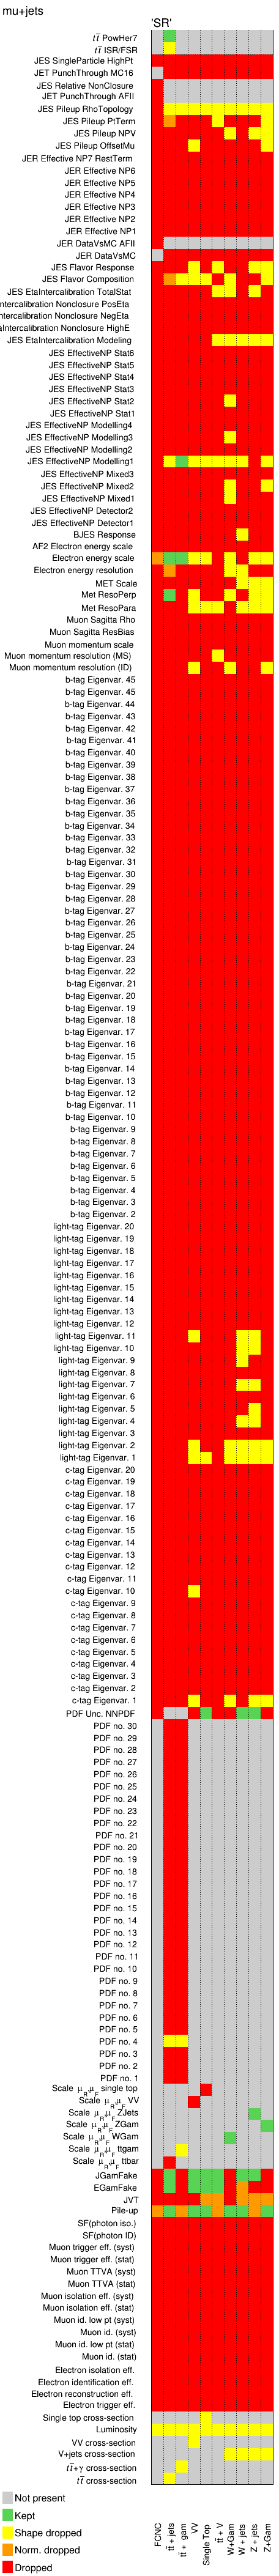
\includegraphics[width=.5\columnwidth]{../ThesisImages/RegionPlots/FinalRegions/Systematics/MQGamEJetPHptMJet/FCNC_All_mujets/Pruning.png}
	\caption[Nuisance parameters after pruning for $\mu$+jets channel]{Overview of nuisance parameters after pruning for the $\mu$+jets channel.  If shape or normalization impacts are smaller than 1\% that part of the nuisance parameter will be dropped in the final fit. }
	\label{fig:Pruningmujets}
\end{figure}

\begin{figure}[h!]
	\centering
	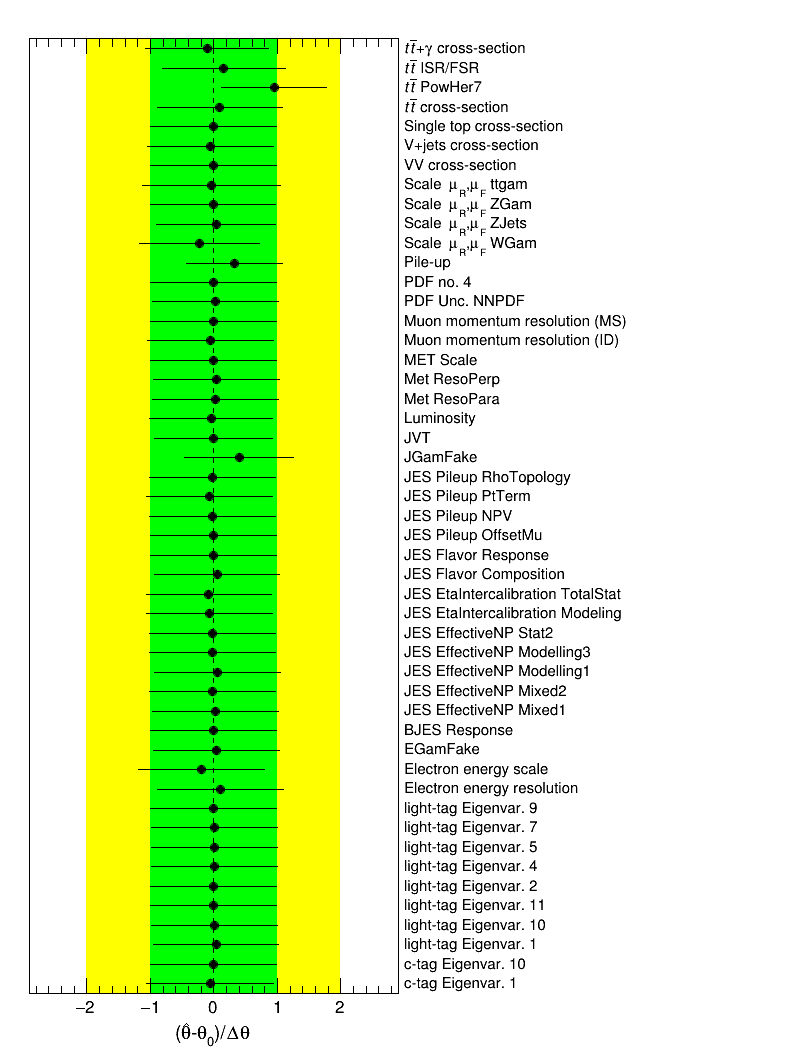
\includegraphics[width=.5\columnwidth]{../ThesisImages/RegionPlots/FinalRegions/Systematics/MQGamEJetPHptMJet/FCNC_All_mujets/NuisPar.png}
	\caption{Pull values for the various nuisance parameters considered in the fit for the $\mu$+jets channel.}
	\label{fig:NPmujets}
\end{figure}

\begin{figure}[h!]
	\centering
	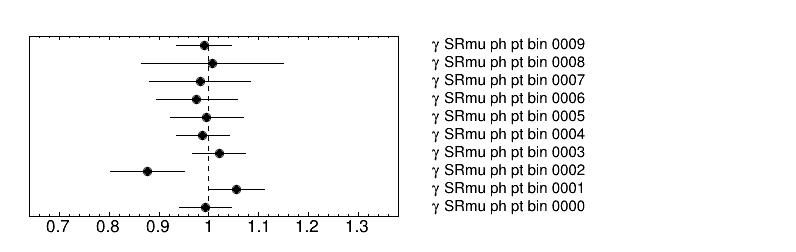
\includegraphics[width=.5\columnwidth]{../ThesisImages/RegionPlots/FinalRegions/Systematics/MQGamEJetPHptMJet/FCNC_All_mujets/Gammas.png}
	\caption{Bin by bin normalization $\gamma$ factors used in each region for the $\mu$+jets channel.}
	\label{fig:Gammasmujets}
\end{figure}

\begin{figure}[h!]
	\centering
	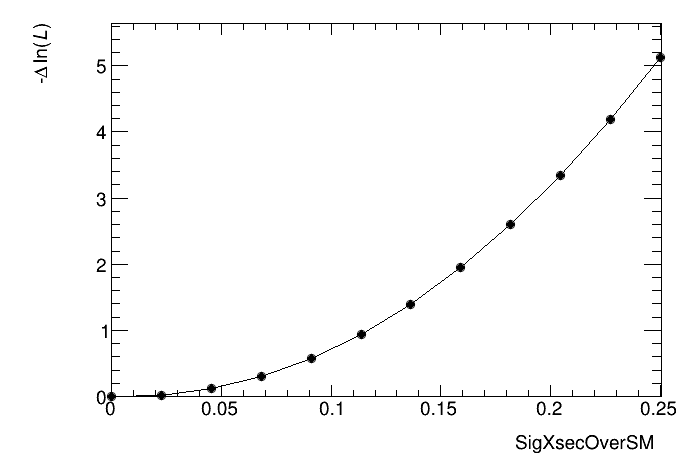
\includegraphics[width=.5\columnwidth]{../ThesisImages/RegionPlots/FinalRegions/Systematics/MQGamEJetPHptMJet/FCNC_All_mujets/LHoodPlots/NLLscan_SigXsecOverSM.png}
	\caption{Negative-log likelihood (goodness of fit) as a function of signal strength using data in all regions for the $\mu$+jets channel.}
	\label{fig:NLLmujets}
\end{figure}

\begin{figure}[h!]
	\centering
	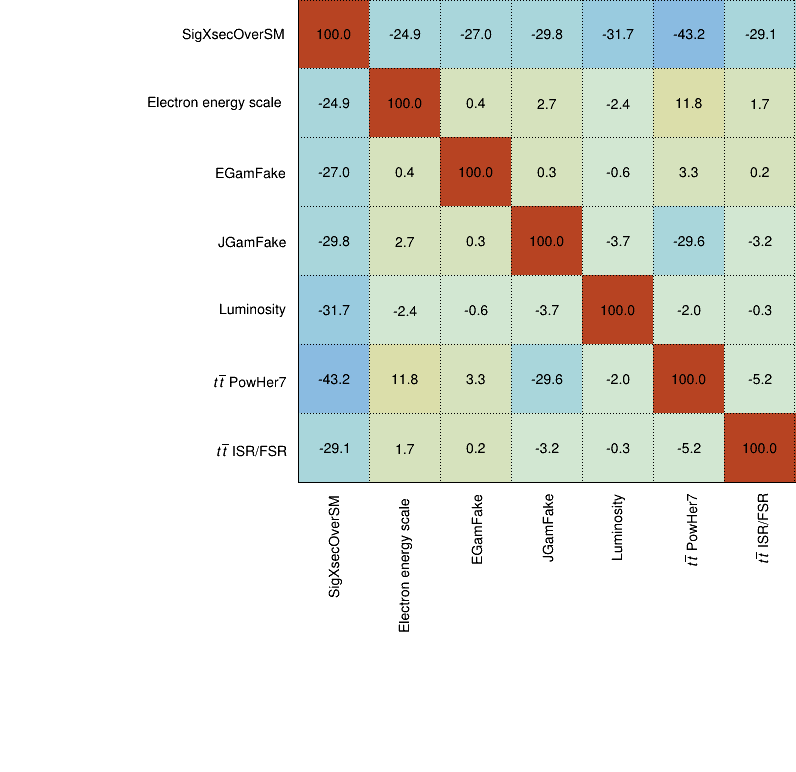
\includegraphics[width=.5\columnwidth]{../ThesisImages/RegionPlots/FinalRegions/Systematics/MQGamEJetPHptMJet/FCNC_All_mujets/CorrMatrix.png}
	\caption[Correlation matrix  with at least one coefficient above 20\% for $\mu$+jets channel]{Correlation matrix  with at least one coefficient above 20\% for $\mu$+jets channel. }
	\label{fig:Corrmujets}
\end{figure}
% Change - Add Ranking Plots

\section{Post-fit Signal Region Plots}
\label{sec:PostFitSR}
Every variable distribution contains shape information and as such will have slight differences in the final limit value after fitting the distributions including variations from the nuisance parameters.  Simultaneous fits are done on well-modeled variables with largest separation, as shown in Table \ref{tab:Separations}.  In addition to these separate fits combinations of fits are done and the best results are presented in this section.  Further fit results are presented in Appendix \ref{app:AddFits}. The variable with the best tested fit for the e+jets signal region is the invariant mass of the up type quark and the photon, $m_{q\gamma}$, which is near the mass of the top quark for the FCNC mode being searched for. The variable with the best tested fit for the $\mu$+jets signal region is the transverse momentum of the photon.  The post-fit effects of all systematics are listed in Appendix \ref{app:Syst_Eff} (Tables \ref{tab:ejetsSyst} and \ref{tab:mujetsSyst}).

\begin{figure}[]
\centering
\subfloat[]{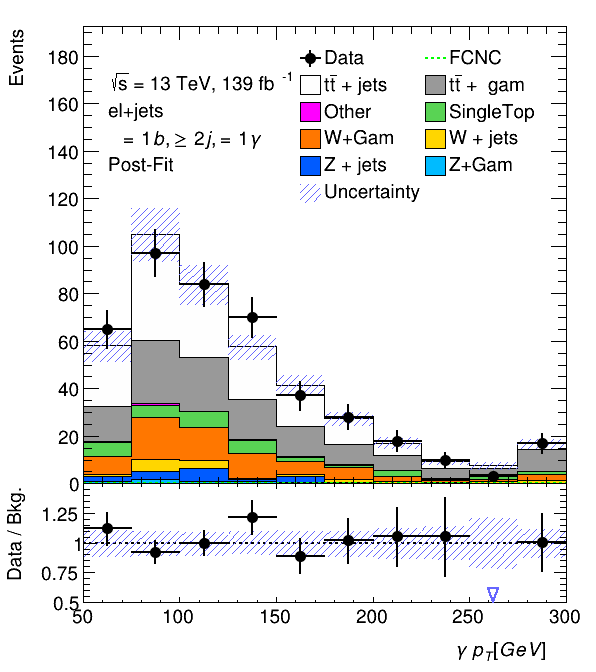
\includegraphics[width=.33\columnwidth]{../ThesisImages/RegionPlots/FinalRegions/Systematics/MQGamEJetPHptMJet/FCNC_All_ejets/Plots/SR_ph_pt_postFit.png}}\hfil
\subfloat[]{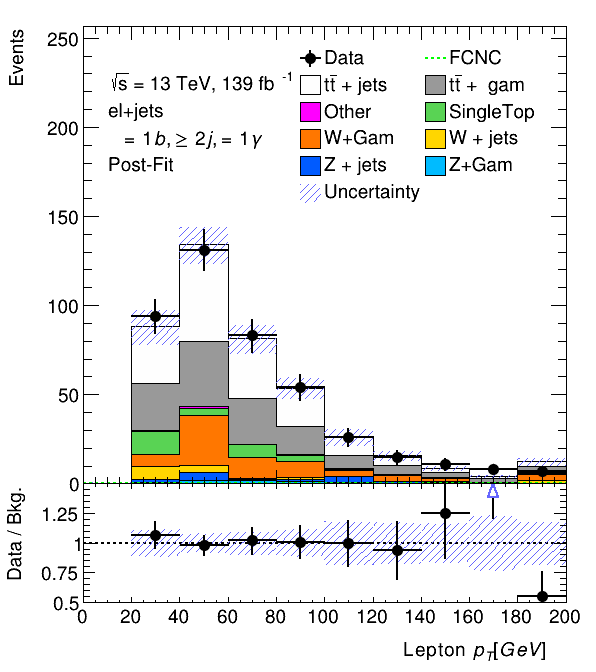
\includegraphics[width=.33\columnwidth]{../ThesisImages/RegionPlots/FinalRegions/Systematics/MQGamEJetPHptMJet/FCNC_All_ejets/Plots/SR_lep_pt_postFit.png}}\hfil  
\subfloat[]{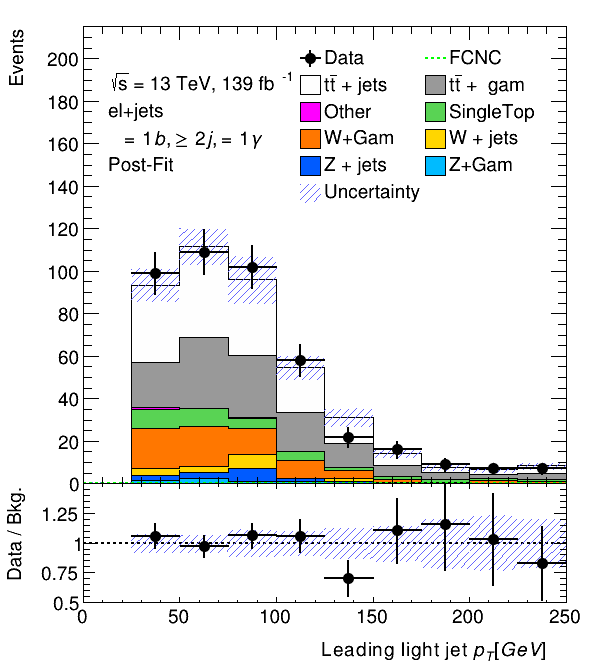
\includegraphics[width=.33\columnwidth]{../ThesisImages/RegionPlots/FinalRegions/Systematics/MQGamEJetPHptMJet/FCNC_All_ejets/Plots/SR_jet0_pt_postFit.png}}
\vspace{-3.mm}
\subfloat[]{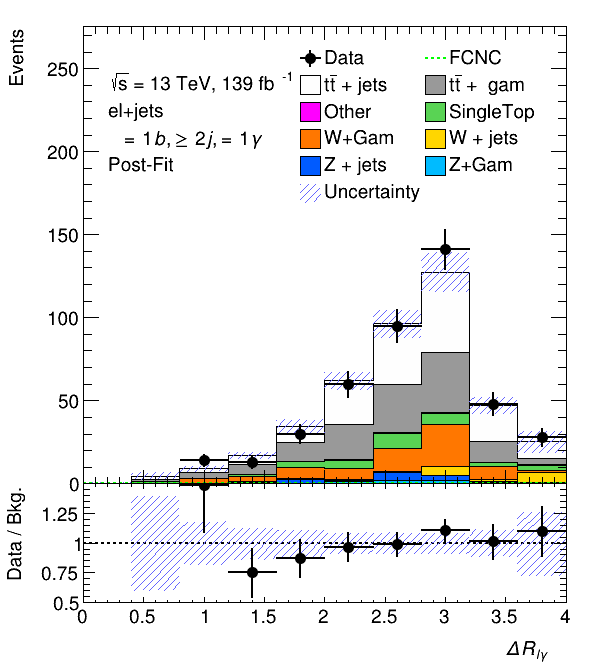
\includegraphics[width=.33\columnwidth]{../ThesisImages/RegionPlots/FinalRegions/Systematics/MQGamEJetPHptMJet/FCNC_All_ejets/Plots/SR_drlph_postFit.png}}\hfil
\subfloat[]{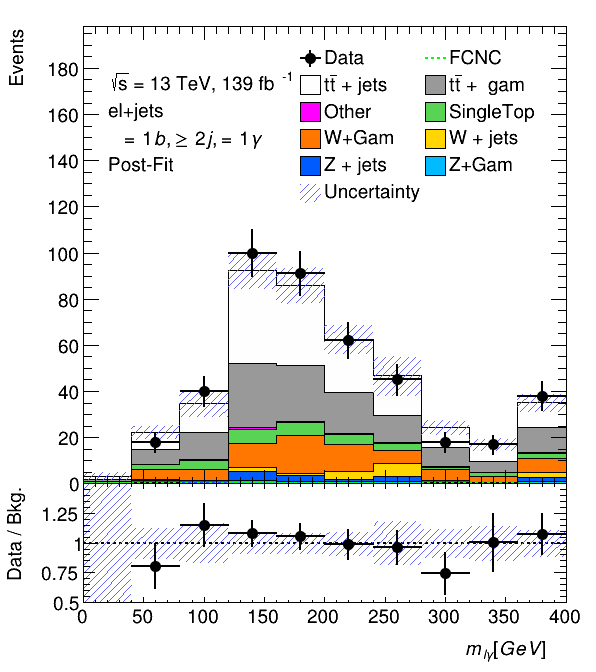
\includegraphics[width=.33\columnwidth]{../ThesisImages/RegionPlots/FinalRegions/Systematics/MQGamEJetPHptMJet/FCNC_All_ejets/Plots/SR_m_lgam_postFit.png}}\hfil  
\subfloat[]{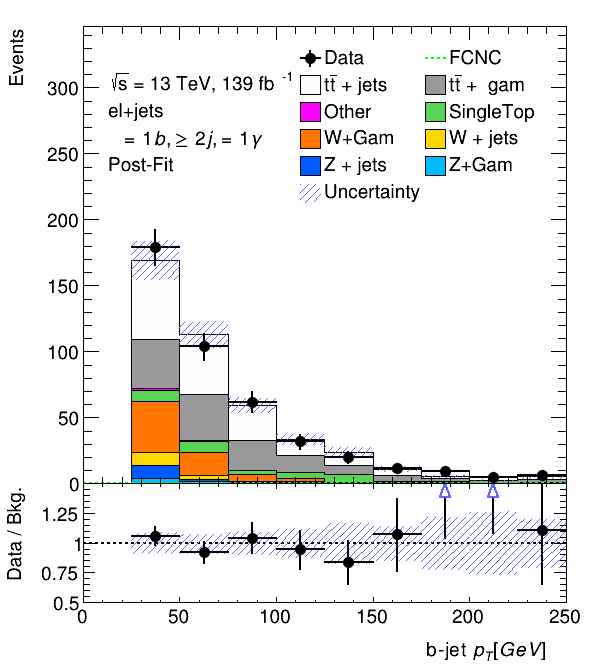
\includegraphics[width=.33\columnwidth]{../ThesisImages/RegionPlots/FinalRegions/Systematics/MQGamEJetPHptMJet/FCNC_All_ejets/Plots/SR_bjet0_pt_postFit.png}}
\caption{Post-fit distributions for Photon $p_T$ (a), lepton $p_T$ (b), leading light jet $p_T$ (c), $\Delta R_{l\gamma}$ (d), $m_{l \gamma}$ (e), and b-jet $p_T$ (f) in the final signal region for the electron channel. }
\label{fig:fitSRej1}
\end{figure}


\begin{figure}[]
\centering
\subfloat[]{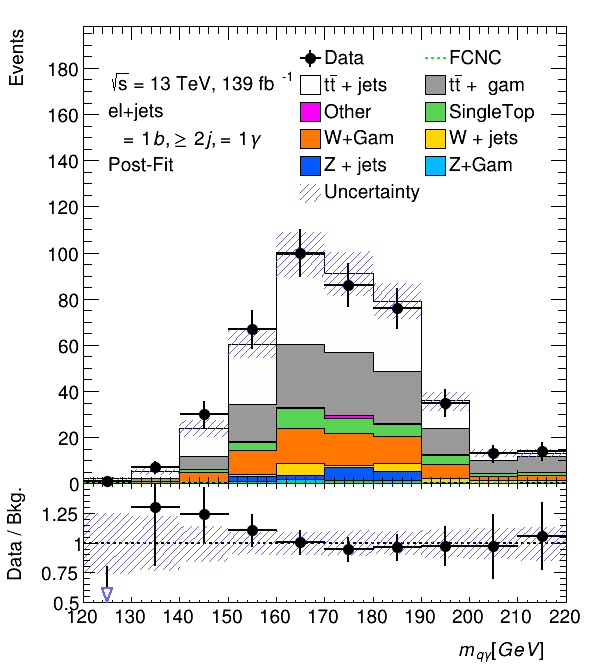
\includegraphics[width=.33\columnwidth]{../ThesisImages/RegionPlots/FinalRegions/Systematics/MQGamEJetPHptMJet/FCNC_All_ejets/Plots/SR_mqph_postFit.png}}\hfil
\subfloat[]{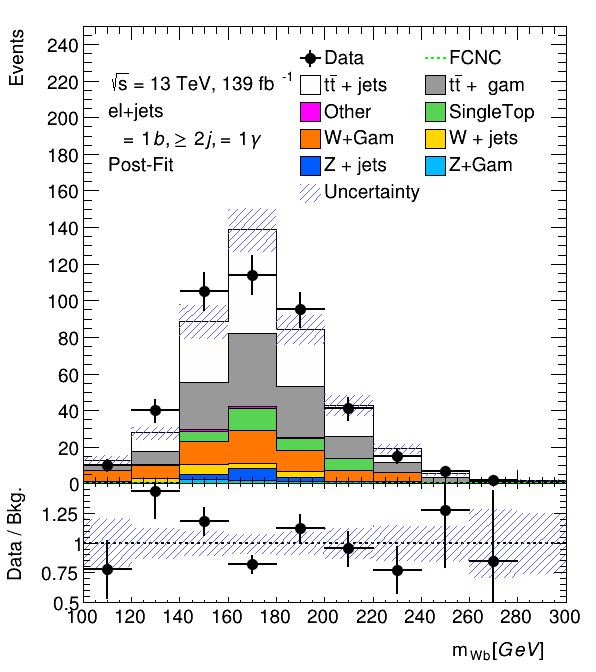
\includegraphics[width=.33\columnwidth]{../ThesisImages/RegionPlots/FinalRegions/Systematics/MQGamEJetPHptMJet/FCNC_All_ejets/Plots/SR_SMtop_postFit.png}}\hfil  
\subfloat[]{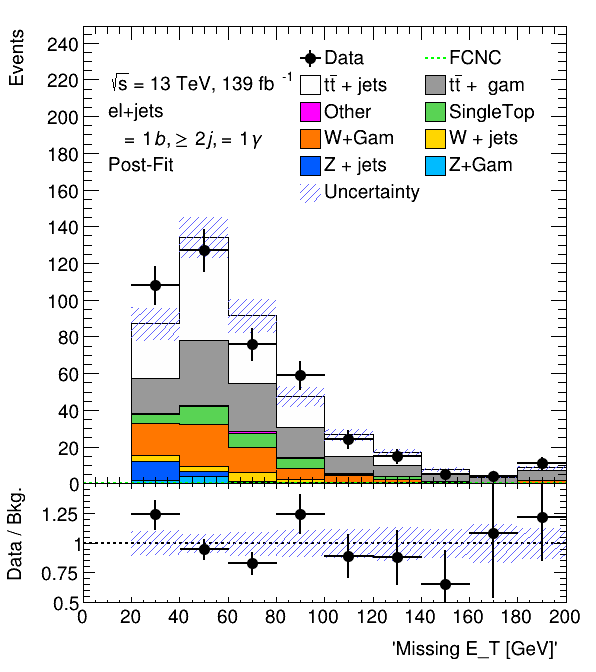
\includegraphics[width=.33\columnwidth]{../ThesisImages/RegionPlots/FinalRegions/Systematics/MQGamEJetPHptMJet/FCNC_All_ejets/Plots/SR_met_postFit.png}}
\vspace{-3.mm}
\subfloat[]{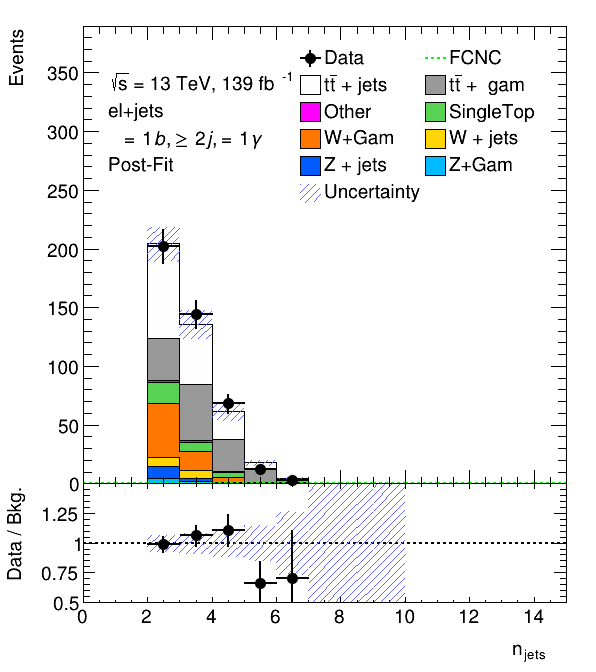
\includegraphics[width=.33\columnwidth]{../ThesisImages/RegionPlots/FinalRegions/Systematics/MQGamEJetPHptMJet/FCNC_All_ejets/Plots/SR_njet_postFit.png}}\hfil
\subfloat[]{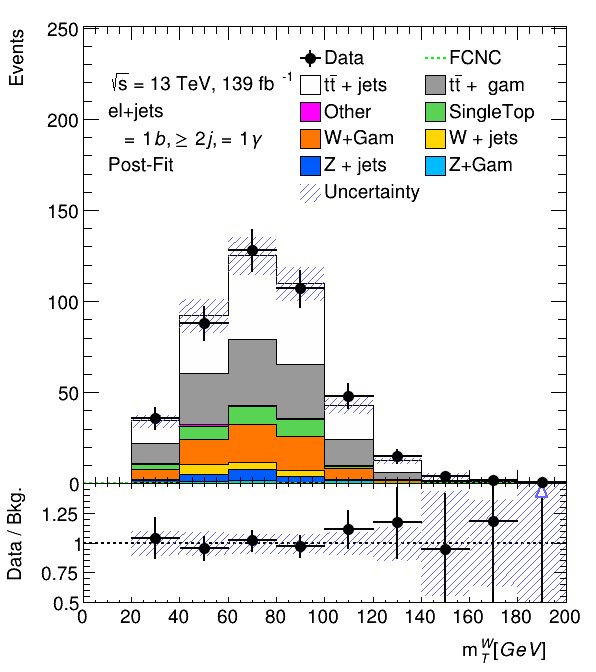
\includegraphics[width=.33\columnwidth]{../ThesisImages/RegionPlots/FinalRegions/Systematics/MQGamEJetPHptMJet/FCNC_All_ejets/Plots/SR_MWT_postFit.png}}\hfil  
\subfloat[]{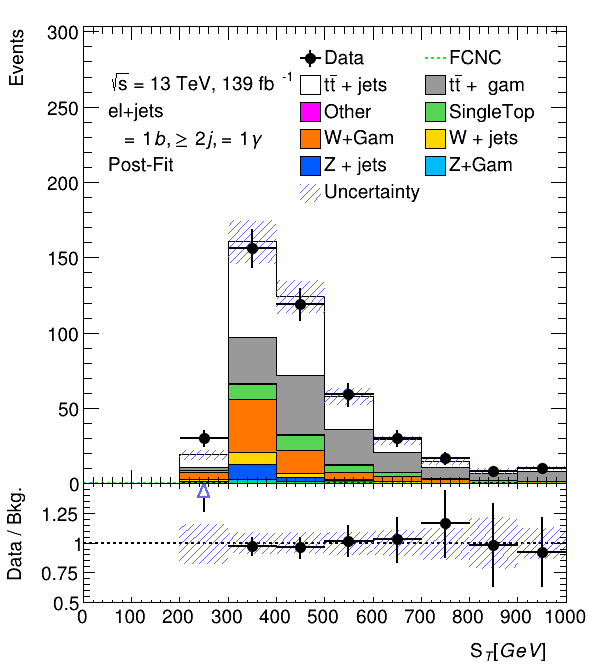
\includegraphics[width=.33\columnwidth]{../ThesisImages/RegionPlots/FinalRegions/Systematics/MQGamEJetPHptMJet/FCNC_All_ejets/Plots/SR_ST_postFit.png}}
\caption{Post-fit distributions for FCNC top candidate mass (a), Standard Model top candidate mass (b), $\slashed{E}_T$ (c), $N_\text{jets}$ (d),  $m_T^W$ (e), and $S_T$ (f) in the final signal region for the electron channel.}
\label{fig:fitSRej2}
\end{figure}


\begin{figure}[]
\centering
\subfloat[]{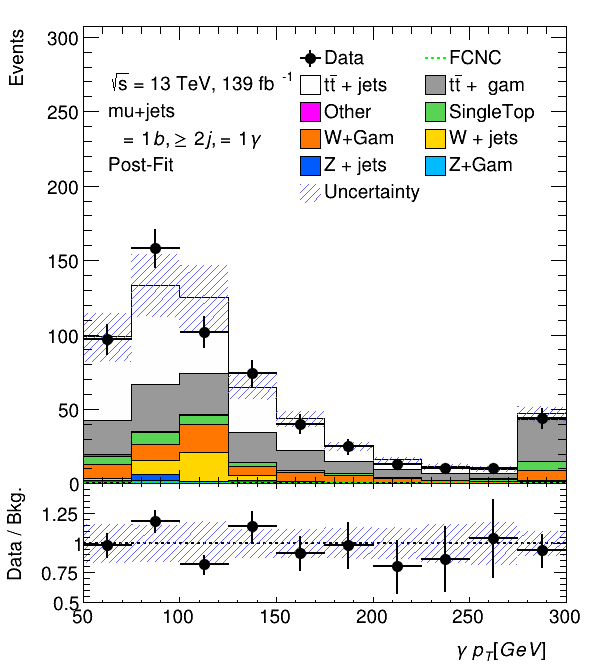
\includegraphics[width=.33\columnwidth]{../ThesisImages/RegionPlots/FinalRegions/Systematics/MQGamEJetPHptMJet/FCNC_All_mujets/Plots/SRmu_ph_pt_postFit.png}}\hfil
\subfloat[]{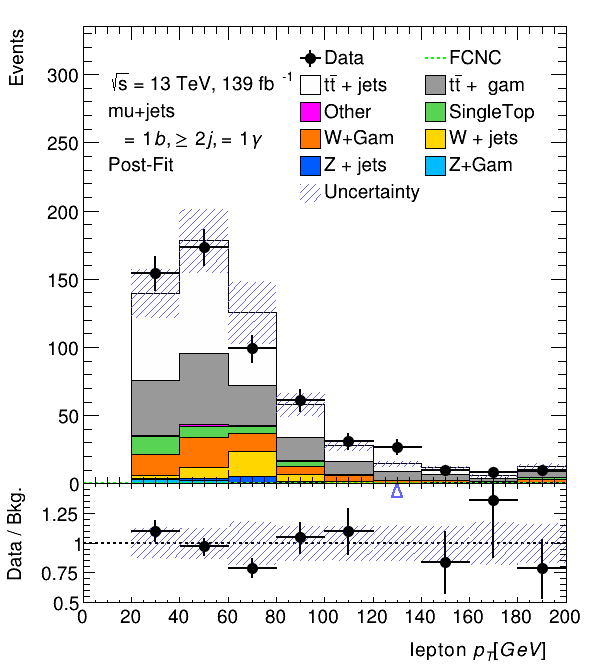
\includegraphics[width=.33\columnwidth]{../ThesisImages/RegionPlots/FinalRegions/Systematics/MQGamEJetPHptMJet/FCNC_All_mujets/Plots/SRmu_lep_pt_postFit.png}}\hfil  
\subfloat[]{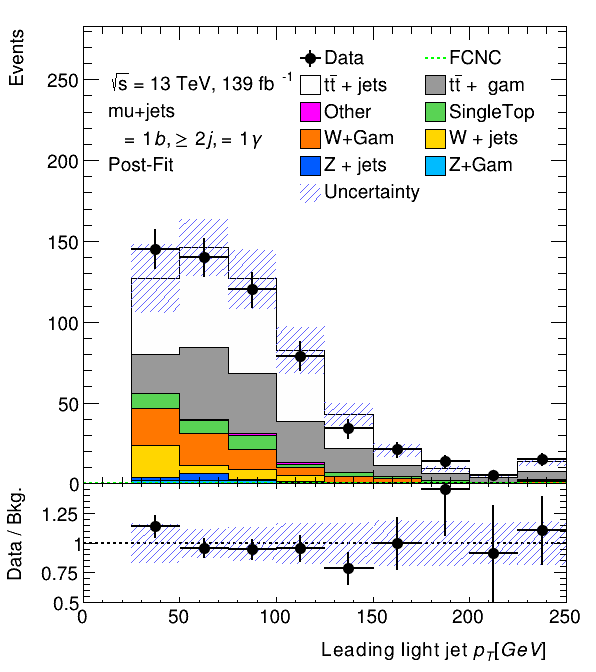
\includegraphics[width=.33\columnwidth]{../ThesisImages/RegionPlots/FinalRegions/Systematics/MQGamEJetPHptMJet/FCNC_All_mujets/Plots/SRmu_jet0_pt_postFit.png}}
\vspace{-3.mm}
\subfloat[]{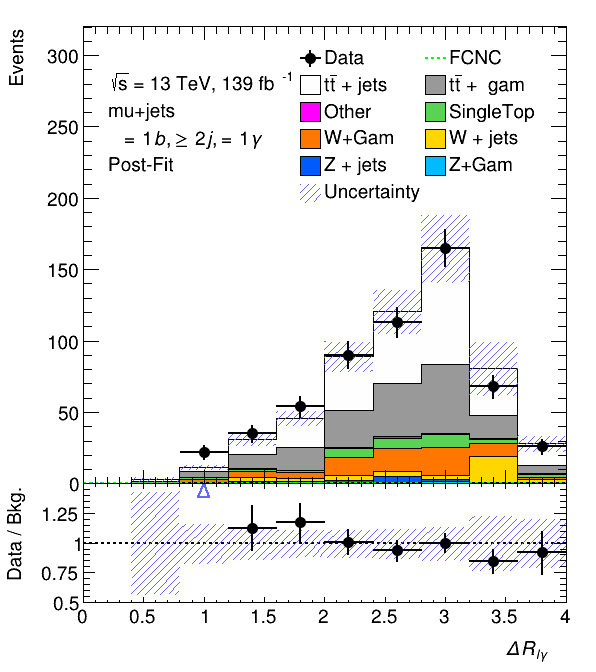
\includegraphics[width=.33\columnwidth]{../ThesisImages/RegionPlots/FinalRegions/Systematics/MQGamEJetPHptMJet/FCNC_All_mujets/Plots/SRmu_drlph_postFit.png}}\hfil
\subfloat[]{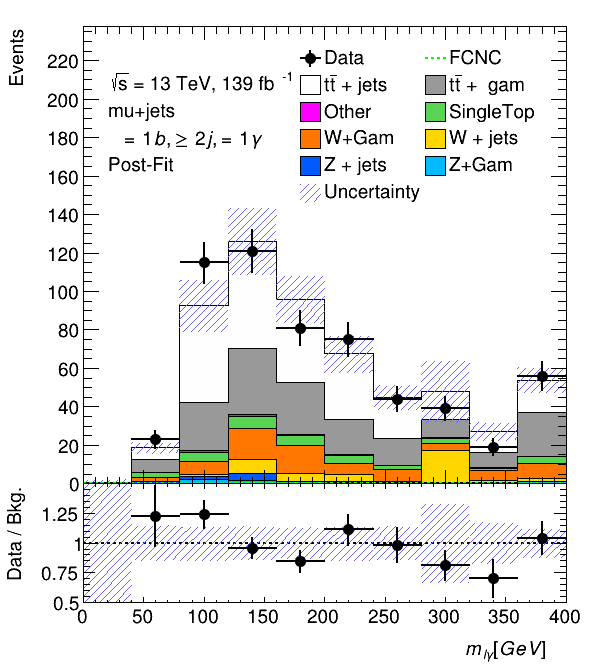
\includegraphics[width=.33\columnwidth]{../ThesisImages/RegionPlots/FinalRegions/Systematics/MQGamEJetPHptMJet/FCNC_All_mujets/Plots/SRmu_m_lgam_postFit.png}}\hfil  
\subfloat[]{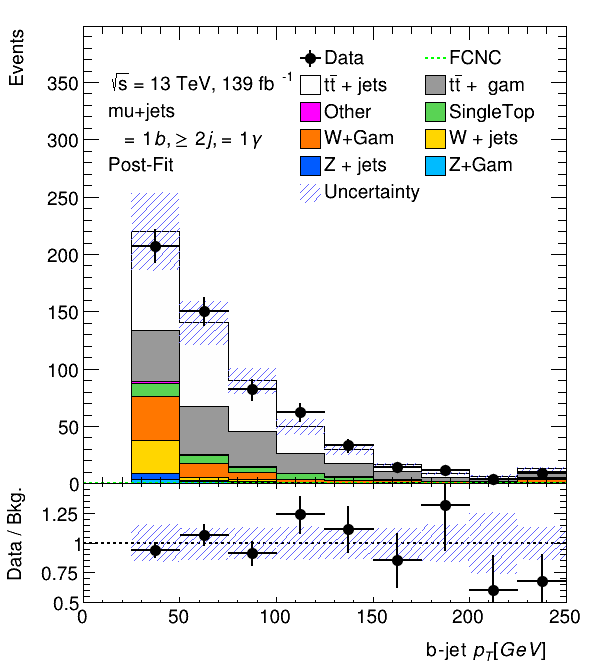
\includegraphics[width=.33\columnwidth]{../ThesisImages/RegionPlots/FinalRegions/Systematics/MQGamEJetPHptMJet/FCNC_All_mujets/Plots/SRmu_bjet0_pt_postFit.png}}
\caption{Post-fit distributions for Photon $p_T$ (a), lepton $p_T$ (b), leading light jet $p_T$ (c), $\Delta R_{l\gamma}$ (d), $m_{l \gamma}$ (e), and b-jet $p_T$ (f) in the final signal region for the muon channel.}
\label{fig:fitSRmuj1}
\end{figure}


\begin{figure}[]
\centering
\subfloat[]{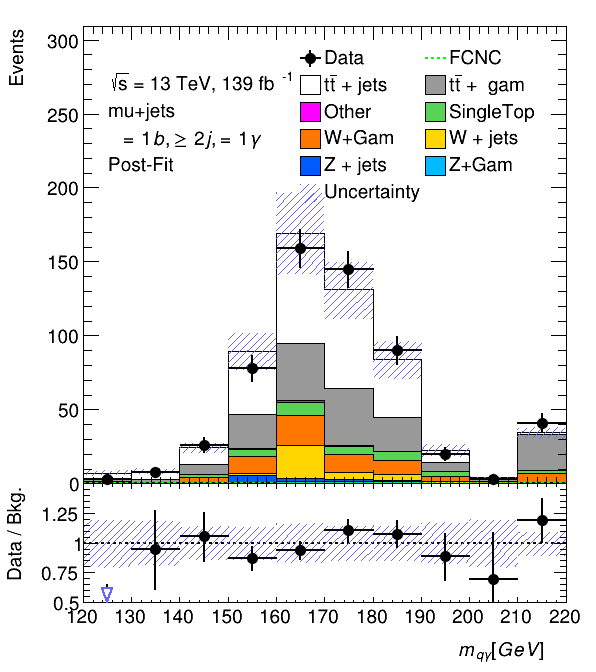
\includegraphics[width=.33\columnwidth]{../ThesisImages/RegionPlots/FinalRegions/Systematics/MQGamEJetPHptMJet/FCNC_All_mujets/Plots/SRmu_mqph_postFit.png}}\hfil
\subfloat[]{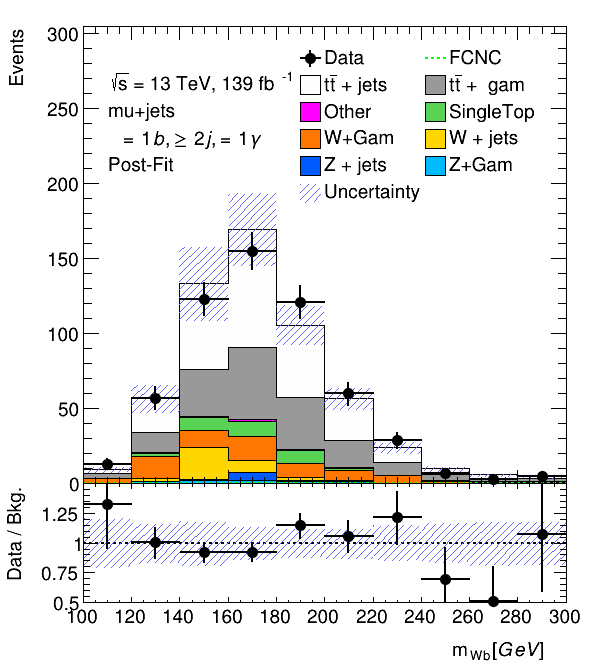
\includegraphics[width=.33\columnwidth]{../ThesisImages/RegionPlots/FinalRegions/Systematics/MQGamEJetPHptMJet/FCNC_All_mujets/Plots/SRmu_SMtop_postFit.png}}\hfil  
\subfloat[]{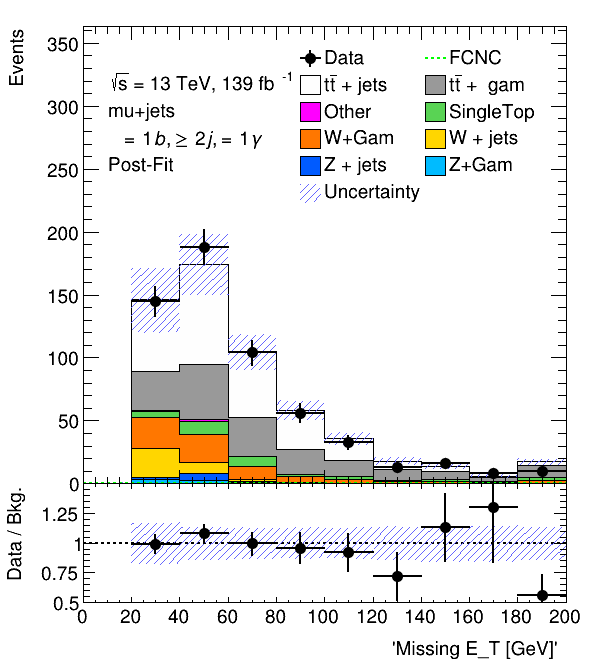
\includegraphics[width=.33\columnwidth]{../ThesisImages/RegionPlots/FinalRegions/Systematics/MQGamEJetPHptMJet/FCNC_All_mujets/Plots/SRmu_met_postFit.png}}
\vspace{-3.mm}
\subfloat[]{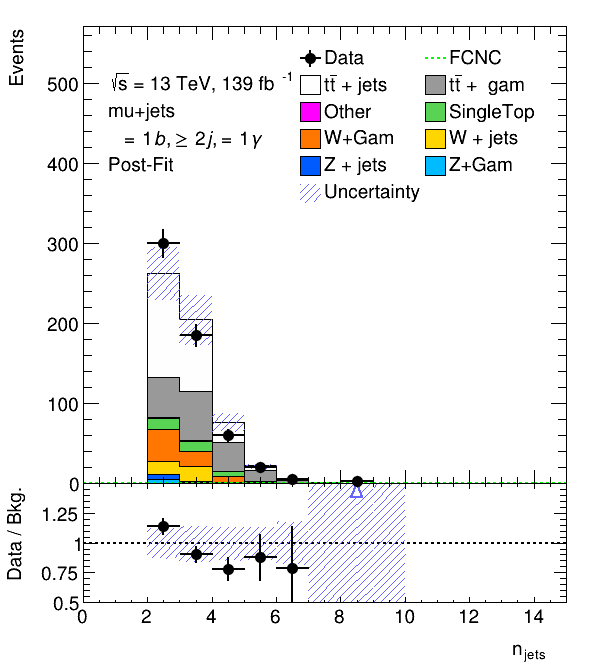
\includegraphics[width=.33\columnwidth]{../ThesisImages/RegionPlots/FinalRegions/Systematics/MQGamEJetPHptMJet/FCNC_All_mujets/Plots/SRmu_njet_postFit.png}}\hfil
\subfloat[]{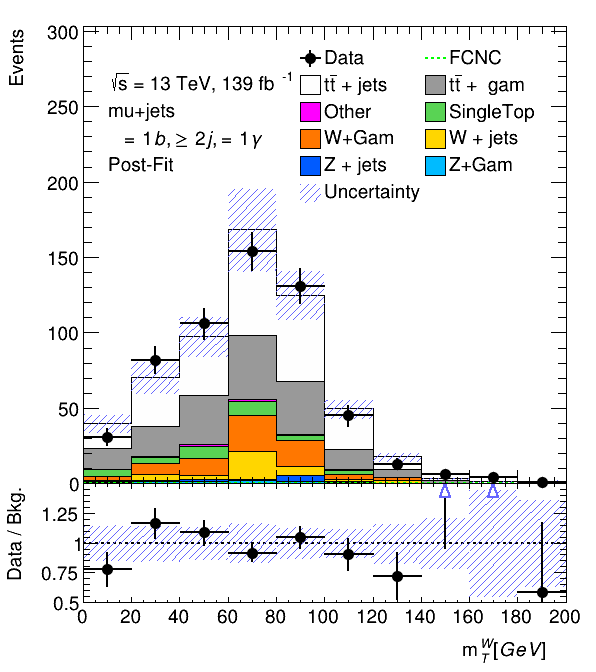
\includegraphics[width=.33\columnwidth]{../ThesisImages/RegionPlots/FinalRegions/Systematics/MQGamEJetPHptMJet/FCNC_All_mujets/Plots/SRmu_MWT_postFit.png}}\hfil  
\subfloat[]{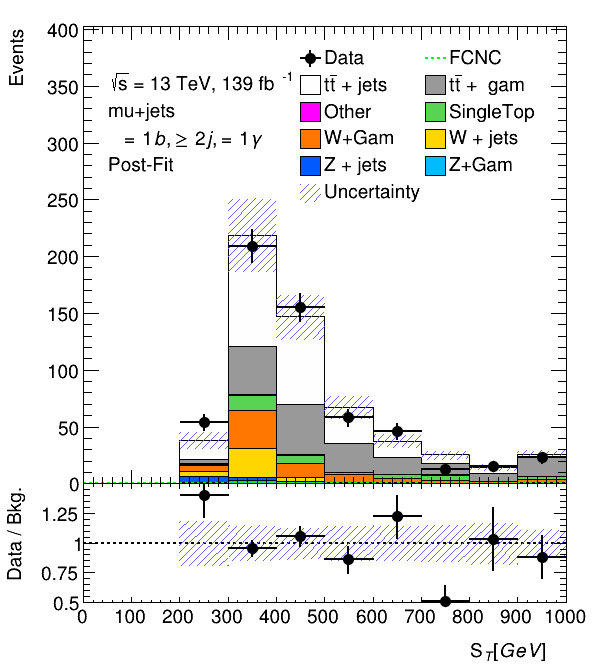
\includegraphics[width=.33\columnwidth]{../ThesisImages/RegionPlots/FinalRegions/Systematics/MQGamEJetPHptMJet/FCNC_All_mujets/Plots/SRmu_ST_postFit.png}}
\caption{Post-fit distributions for FCNC top candidate mass (a), Standard Model top candidate mass (b), $\slashed{E}_T$ (c), $N_\text{jets}$ (d),  $m_T^W$ (e), and $S_T$ (f) in the final signal region for the muon channel.}
\label{fig:fitSRmuj2}
\end{figure}

\subsection{Post-fit Data and MC Yields}
\begin{table}[h!]
\begin{center}
{\renewcommand{\arraystretch}{1.2}
\begin{tabular}{ccc}
\hhline{===}
Sample  &  Events e+jets (Fit on $m_{q\gamma}$ ) & Events $\mu$+jets (Fit on $\gamma p_{T}$)  \\  \hline 
FCNC, signal		& 0.0 $\pm$ 1.7 & 0.6 $\pm$ 7.0\\
$t\bar{t}$            		& 162.9 $\pm$ 30.6 & 253.5 $\pm$ 55.6\\
$t\bar{t}+\gamma$           & 125.1 $\pm$ 12.3 & 165.6 $\pm$ 16.6\\
W+jets			& 14.4 $\pm$ 7.9 & 35.1 $\pm$ 18.5\\   
W+jets+$\gamma$		& 67.1 $\pm$ 15.3 & 68.6 $\pm$ 14.6\\
Z+jets	            	& 13.9 $\pm$ 5.6 & 8.0 $\pm$ 4.7\\
Z+jets+$\gamma$		& 7.2 $\pm$ 3.6 & 8.4 $\pm$ 2.6\\
Single top 		           & 31.4 $\pm$ 6.7 & 33.0 $\pm$ 6.4\\
Diboson (VV)		          	& 1.7 $\pm$ 0.7 & 2.1 $\pm$ 0.8\\
$t\bar{t}+V$	           & 1.2 $\pm$ 0.2 & 1.6 $\pm$ 0.3 \\ \hline
Total MC 			& 424.9 $\pm$ 29.3 & 575.9 $\pm$ 72.9\\ \hline
Data		                     	& 429 & 573\\ \hhline{===}
\end{tabular}
\caption{Post-fit signal region event yields.}
\label{tab:postfitSRYields}
}
\end{center}
\end{table}



\section{Limit on Branching Ratio t$\rightarrow$q$\gamma$}
\label{sec:Limits}
Limits are calculated using the $CL_\text{s}$ method to place an upper bound on the signal strength, $\mu$.  This signal strength can then be interpreted as a branching ratio or a cross section by comparing to the nominal value used for signal simulation as discussed in Section \ref{sec:StatTreatment}.  Table \ref{tab:UpperLimitsMu} shows the 95\% confidence limit on the signal strength and the interpretations in terms of the branching ratio and cross section are shown in Table \ref{tab:UpperLimitsBR} and Table \ref{tab:UpperLimitsXS}, respectively. Figure \ref{fig:UpperLimMu} shows the observed upper limits for the signal strength.
%Combining searches with small stats from Lizas: \cite{Junk:1999kv}
\begin{table}[h!]
\begin{center}
{\renewcommand{\arraystretch}{1.2}
\begin{tabular}{ccccc}
\hhline{=====}
Channel  	&  Obs. Limit			&	Exp. Limit -$\sigma$	& Exp. Limit	& Exp. Limit +$\sigma$  \\  \hline 
e+jets	& $0.119$ 	& $0.094$	& $0.131$ & $0.178$	\\ 
$\mu$+jets	& $0.153$ 	& $0.103$	& $0.142$ & $0.193$	\\ 
Combined	& $0.096$ 	& $0.080$	& $0.110$ & $0.153$	\\
\hhline{=====}
\end{tabular}
\caption{Expected and observed upper limits on signal strength $\mu$ used in the fit.}
\label{tab:UpperLimitsMu}
}
\end{center}
\end{table}


\begin{table}[h!]
\begin{center}
{\renewcommand{\arraystretch}{1.2}
\begin{tabular}{ccccc}
\hhline{=====}
Channel  	&  Obs. Limit			&	Exp. Limit -$\sigma$	& Exp. Limit	& Exp. Limit +$\sigma$  \\  \hline 
e+jets	& $1.19\times10^{-4}$ 	& $0.94\times10^{-4}$	& $1.31\times10^{-4}$ & $1.78\times10^{-4}$	\\ 
$\mu$+jets	& $1.53\times10^{-4}$ 	& $1.03\times10^{-4}$	& $1.42\times10^{-4}$ & $1.93\times10^{-4}$	\\ 
Combined	& $0.96\times10^{-4}$ 	& $0.80\times10^{-4}$	& $1.10\times10^{-4}$ & $1.53\times10^{-4}$	\\
\hhline{=====}
\end{tabular}
\caption{Upper limits on the branching ratio BR(t$\rightarrow q \gamma$).}
\label{tab:UpperLimitsBR}
}
\end{center}
\end{table}

\begin{table}[h!]
\begin{center}
{\renewcommand{\arraystretch}{1.2}
\begin{tabular}{ccc}
\hhline{===}
Channel  	&  Obs. Limit	& Exp. Limit	 \\  \hline 
e+jets	& 64 fb	& 71 fb 	\\ 
$\mu$+jets	& 83 fb	& 77 fb 	\\ 
Combined	& 50 fb	& 60 fb 	\\
\hhline{===}
\end{tabular}
\caption{Observed and expected limits on the cross section $\sigma(pp\rightarrow tt \rightarrow Wb q \gamma$).}
\label{tab:UpperLimitsXS}
}
\end{center}
\end{table}

\begin{figure}[ht!]
	\centering
	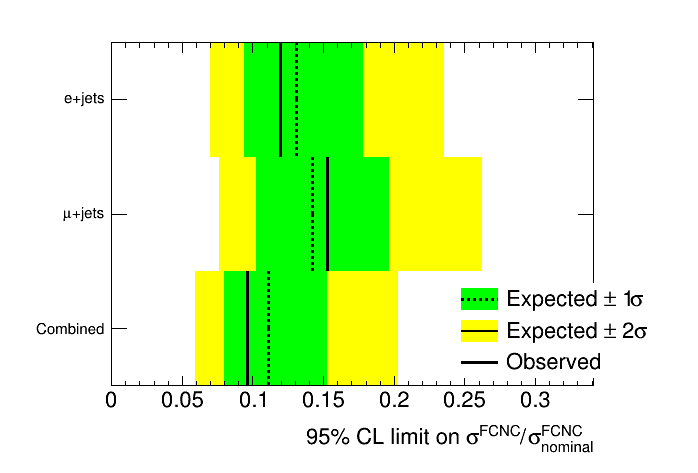
\includegraphics[width=0.5\columnwidth]{../ThesisImages/RegionPlots/FinalRegions/Systematics/MQGamEJetPHptMJet/LimitPlot.png}
	\caption{95\% confidence level upper limits on the signal strength $\mu$.
	}
	\label{fig:UpperLimMu}
\end{figure}
%
%%%%%%%%%%%%%%%%%%%%%%%%%%%%%%%%%%%%%%%%%%%%%%%%
%This chapter contains co-authored material from Ref.~\cite{Dijet2017}, written as part of the ATLAS Collaboration.
%\newline